\section{课题来源及研究的目的和意义}
\subsection{课题来源}
随着网络通信技术的快速进步和信息技术的普遍应用,互联网上的信息交换变得极为频繁,每时每刻都有大量的数据在网络中流动。这些数据的公开性极大地增加了网络风险。面对这种日益复杂的网络威胁,众多网络安全公司利用现有的威胁情报和数据进行分析,开发了多种入侵检测和响应措施。但是,现有的网络安全防护措施常常依赖于来自不同来源和格式的数据(例如安全警报、网络数据流、安全分析报告和服务器日志等),这些数据难以被统一和结构化,导致在进行关联分析和深入评估时存在明显的缺陷。尽管现有的大语言模型在处理通用知识问答方面表现出色,但在特定领域,尤其是网络安全领域,其性能仍有待提升。特别是在病毒检测等专业领域,大语言模型往往难以准确理解和生成与网络安全相关的问答内容。

网络安全领域的问答系统需要具备高度的专业性和准确性,这对于模型的理解能力和生成能力提出了更高的要求。现有的大语言模型虽然在自然语言处理方面取得了显著进展,但在特定领域的深度理解和知识生成方面仍存在局限。为了提高模型在网络安全问答中的性能,本研究提出了引入奖励模型的方法,旨在通过奖励机制来引导模型生成更高质量、更具领域相关性的问答内容。

本研究的探索需求在于,如何有效地利用大语言模型在网络安全问答生成中的应用,并通过奖励模型的引入,提升问答系统在网络安全领域的专业性和准确性。通过这一研究,我们期望能够开发出更加智能、高效的网络安全问答系统,以应对日益严峻的网络安全挑战。
\subsection{研究目的和意义}
本研究的目的在于实现大语言模型在网络安全问答生成中的优化。具体而言,通过引入奖励模型,我们旨在提升目标模型的专业性、回答的准确性以及对用户需求的响应能力。此外,本研究还旨在构建一个自动反馈系统,该系统能够在网络安全领域提供高质量、可靠的问答服务,以满足日益增长的网络安全信息需求。

基于奖励模型对大模型的调优过程的重要实践意义,我们的研究目标设定为:
\begin{itemize}
    \item[1.] \textbf{高质量数据集的构建:}传统的数据集构架方式是通过人工方式收集数据,例如MNIST数据集就是通过从高中生和人口普查局员工中收集手写数字图像构建的。但是人工收集数据集的缺点在于它通常耗时耗力,成本较高,且容易受到人为偏差的影响。由于需要大量的人力投入,这个过程往往效率低下。此外,人工标注数据可能会引入错误和不一致性,影响数据集的准确性和可靠性。随着数据量的增加,人工收集和标注的难度和复杂性也会显著增加,这限制了数据集的规模和多样性。因此,人工收集数据集在处理大规模、复杂或需要快速更新的场景时存在明显的局限性。本课题通过使用网络安全文本输入Bonito模型自动生成问答对可以大大提升速度与成本收益,并且Bonito模型作为轻量化已开源的模型,对Bonito模型调整后处理数据集构建的任务将减少人员负担。
    \item[2.] \textbf{奖励模型的指令微调:}RLHF中使用的模型数据会受到各种复杂主观因素的影响,包括生成示范数据的人工标注者的偏好、设计研究并编写标签说明的研究人员的偏好,以及由开发人员编写或客户提供的提示,由于人类的偏好并不一致,这可能导致模型在不同情境下的表现不一致。而奖励模型可以自动化地为目标模型的训练提供评分标量,无需每次都依赖人类的直接反馈,这大大提高了对目标模型的训练过程的效率和可扩展性。
    \item[3.] \textbf{目标模型的反馈调整:}在目标模型的任务中,原本的网络安全的问题由人工解决可能会出现误判现象或者收到误导从而导致误报或漏报的情况发生。而最后的目标模型会将根据奖励模型给出的评分策略从而选择更加接近正确结果的回答,其在效率、准确性、考虑范围等方面相对于传统的人工判断会有很大的提升。
\end{itemize}

\section{国内外在该方向的研究现状及分析}
\subsection{国际研究现状}
为了解决人类反馈在生成式模型的调整中的种种局限性,国外的研究者提出了RLHF、RLAIF、RLHF与RLAIF的混合方法以及谷歌提出的GenRM生成式验证器。
\subsubsection{RLHF方法}
通过强化学习(RL)框架,特别是近端策略优化(PPO)算法,来微调的语言模型,其行为更符合人类反馈所指示的偏好。在TruthfulQA基准测试中\cite{ouyang2022training},InstructGPT(RLHF框架下的大模型)生成真实和有信息量的回答的频率是GPT-3的两倍,并且在“封闭领域”任务中,InstructGPT模型捏造信息的频率大约是GPT-3的一半(21\%对比41\%的幻觉率)。然而,这一过程资源密集且技术挑战大\cite{mahan2024generative},通常需要大量的人类偏好标签来训练反映人类偏好的奖励模型。
\subsubsection{RLAIF方法}
由于基于人类反馈的局限性,研究者提出了“宪法AI”\cite{bai2022constitutional}(Constitutional AI)的方法,通过结合SL与RF,利用人类指令训练模型,而无需任何人类标签来识别有害输出。然而模型的泛化能力将会是一个问题,尽管在特定任务和数据集上表现出色,但在未见过的任务和领域上的表现仍然是一个未知数。
\subsubsection{RLHF与RLAIF的混合方法}
由于RLHF与RLAIF都有一定的缺陷但是其优点不可忽视,从而提出了两种RLAIF策略\cite{arXiv:2309.00267}:“Distilled RLAIF”和“Direct RLAIF”。在“Distilled RLAIF”中,研究者们遵循传统的RLHF方法,使用偏好来训练一个奖励模型,然后使用这个模型来训练LLM策略。而在“Direct RLAIF”中,研究者们利用LLM反馈,通过提示LLM直接输出评估分数,作为强化学习中策略训练的信号。该方法结合了人类反馈和人工智能反馈来训练大型语言模型。这种方法的核心在于使用RLAIF策略,它不依赖于人类注释,同时提供了吸引人的扩展属性。研究者们比较了RLAIF和RLHF在三个任务上的有效性:摘要生成、有益对话生成和无害对话生成。实验结果表明,RLAIF和RLHF在人类偏好上的表现相当,RLAIF在无害对话生成任务上甚至超过了RLHF。
\subsubsection{GenRM生成式验证器}
在传统领域中,提高大语言模型(LLMs)性能的主流方法是Best-of-N模式,即由LLM生成N个候选解决方案,然后由验证器进行排序并选出最佳方案。然而,基于LLM的验证器通常被训练成判别分类器来为解决方案打分,这限制了它们利用预训练LLMs文本生成能力的可能性,从而提出了用普遍的下一个标记预测目标来训练验证器,同时进行验证和解决方案生成,即生成式验证器\cite{zhang2024generative}(GenRM),GenRM通过训练LLMs使用下一个标记预测目标,联合进行验证和解决方案生成。这种方法使得GenRM能够利用LLMs的文本生成能力,与指令调整无缝集成,并支持思维链推理。这种生成式验证器相比于标准验证器,可以更好地利用LLMs的几个优势:它们可以无缝集成指令调整,支持思维链推理,并且可以通过多数投票在测试时利用额外的计算来提高验证质量。实验数据表明:GenRM在算法和数学推理任务上的表现优于判别式验证器和LLM-as-a-Judge验证器,在使用Best-of-N解决问题的百分比上提高了16-40\%。
\subsection{国内研究现状}
国内关于大模型在网络安全领域应用的研究现状可以从多个方向展开,尤其是在网络安全态势感知、入侵检测、异常检测等领域有长足进展,通过深度学习和注意力机制等技术的融合提升检测精度与效率。
\subsubsection{基于选择性卷积网络的网络安全态势感知}
基于选择性卷积网络的网络安全态势感知研究 孙明伟等人在研究中提出了一种基于选择性卷积网络(SKN)的网络安全态势评估与预测模型\cite{宋会倩2021基于卷积神经网络的网络安全态势感知研究}。该研究改进了选择性卷积核结构,用以优化特征提取质量,并提出二次分类组合模型,通过分阶段识别和分类攻击,减轻数据不平衡问题。此外,通过融合时域卷积网络(TCN)的选择性时域卷积网络(SKTCN),模型在预测未来网络安全态势的准确性上表现出更高的鲁棒性。该研究利用NSL-KDD、UNSW-NB15和AWID等数据集进行实验,证明了模型在态势评估和预测中的高效性与准确性。
而赵冬梅等提出的研究结合了改进的选择性卷积核和支持向量机(SVM)\cite{SVM的网络安全态势评估},构建了高效的态势评估模型。通过网格优化算法提升分类精度,并在KDDCUP99、UNSW-NB15和N-BaloT数据集上的实验显示,该模型在鲁棒性与准确性方面均优于传统模型,尤其适用于复杂网络环境中的态势评估​。
\subsubsection{基于深度学习的轻量级入侵检测模型与算法}
李泽煜的研究提出了两种入侵检测模型\cite{1023744319.nh}:基于自监督学习的IBYOL-IDS和基于知识蒸馏的轻量级模型(KD-TCNN)。前者利用自监督学习,从无标签数据中提取具有高泛化能力的流量特征,大幅度提升了检测的适应性;后者结合特征选择和卷积网络压缩技术,优化模型复杂度并提升资源受限设备上的检测效率。在多个公开数据集上的实验验证了模型在高维度和不均衡数据上的出色性能。张昊等人的研究\cite{基于深度学习的入侵检测模型综述}总结了卷积神经网络(CNN)、长短期记忆网络(LSTM)、自编码器(AE)以及生成式对抗网络(GAN)在入侵检测中的应用,其中卷积神经网络凭借其权值共享和特征提取能力,能够提升模型的计算效率并减少训练参数。例如,实验表明基于CNN改进的入侵检测模型在KDD99数据集上的准确率达到99.23\%。此外,长短期记忆网络通过捕捉数据间长期依赖关系,适合提取时间序列特征,例如结合CNN的LSTM模型在CIDDS-001数据集上的预测准确率达到97.17\%。
\subsubsection{通过深度学习检测网络异常流量}
基于深度学习的网络异常流量检测研究与系统实现,高嘉提出了创新的研究方法和模型\cite{高嘉2023基于深度学习的网络异常流量检测研究与系统实现}。研究采用基于CNN(卷积神经网络)和GRU(门控循环单元)的时空融合模型,结合注意力机制和自编码器,设计了改进的异常流量检测框架。CNN用于提取网络流量的空间特征,GRU用于捕捉时间序列特性,两者结合以增强数据特征表达能力。此外,通过引入CBAM(卷积块注意力模块)和自编码器,提升模型对重要信息的关注度,同时利用自编码器进行特征压缩,进一步挖掘潜在特性。该方法基于CICIDS-2017数据集进行模型验证显示,在时空融合模型的检测准确率为99.89\%,相比随机森林模型(RF)提高3.21\%,比单独使用CNN和GRU分别提高了0.48\%和0.53\%。优化后的模型结合注意力机制和自编码器后,准确率进一步提升至99.93\%。这表明通过注意力机制增强的深度学习模型在处理复杂网络流量特征时具有明显优势。在杨宏宇团队的总结中,有基于深度学习的网络异常流量检测方法优劣如下\cite{yang2024network}:
\begin{table}[htbp]
    \bicaption[table1]{}{异常流量检测方法总结}{Table$\!$}{Summary of abnormal traffic detection methods}
    \vspace{0.5em}\centering\wuhao
    \begin{tabular}{ccccc}
        \toprule
        检测方法        & 优点          & 缺点           \\
        \midrule
        BiLSTM+特征降维 & 能够有效去除冗余特征  & 模型泛化性较差      \\
        BiLSTM+CNN  & 训练速度快、误报率低  & 对小样本类别的适应性较差 \\
        CNN+RNN     & 检测模型的误报率低   & 模型泛化性较差      \\
        GAN+RF      & 生成流量数据的效果较好 & 模型计算和存储开销大   \\
        HRNN        & 检测模型的误报率低   & 超图构建需要较高计算资源 \\
        \bottomrule
    \end{tabular}
\end{table}
\newpage
\section{主要研究内容}
该研究的主要内容包括:数据收集、Bonito模型生成问答对与指令微调、奖励模型的设计与微调、强化学习与下游神经网络结合调整目标大模型,通过引入奖励模型和指令微调技术,提升目标大语言模型在网络安全问答生成中的专业性和准确性。
\begin{figure}[htbp]
    \centering
    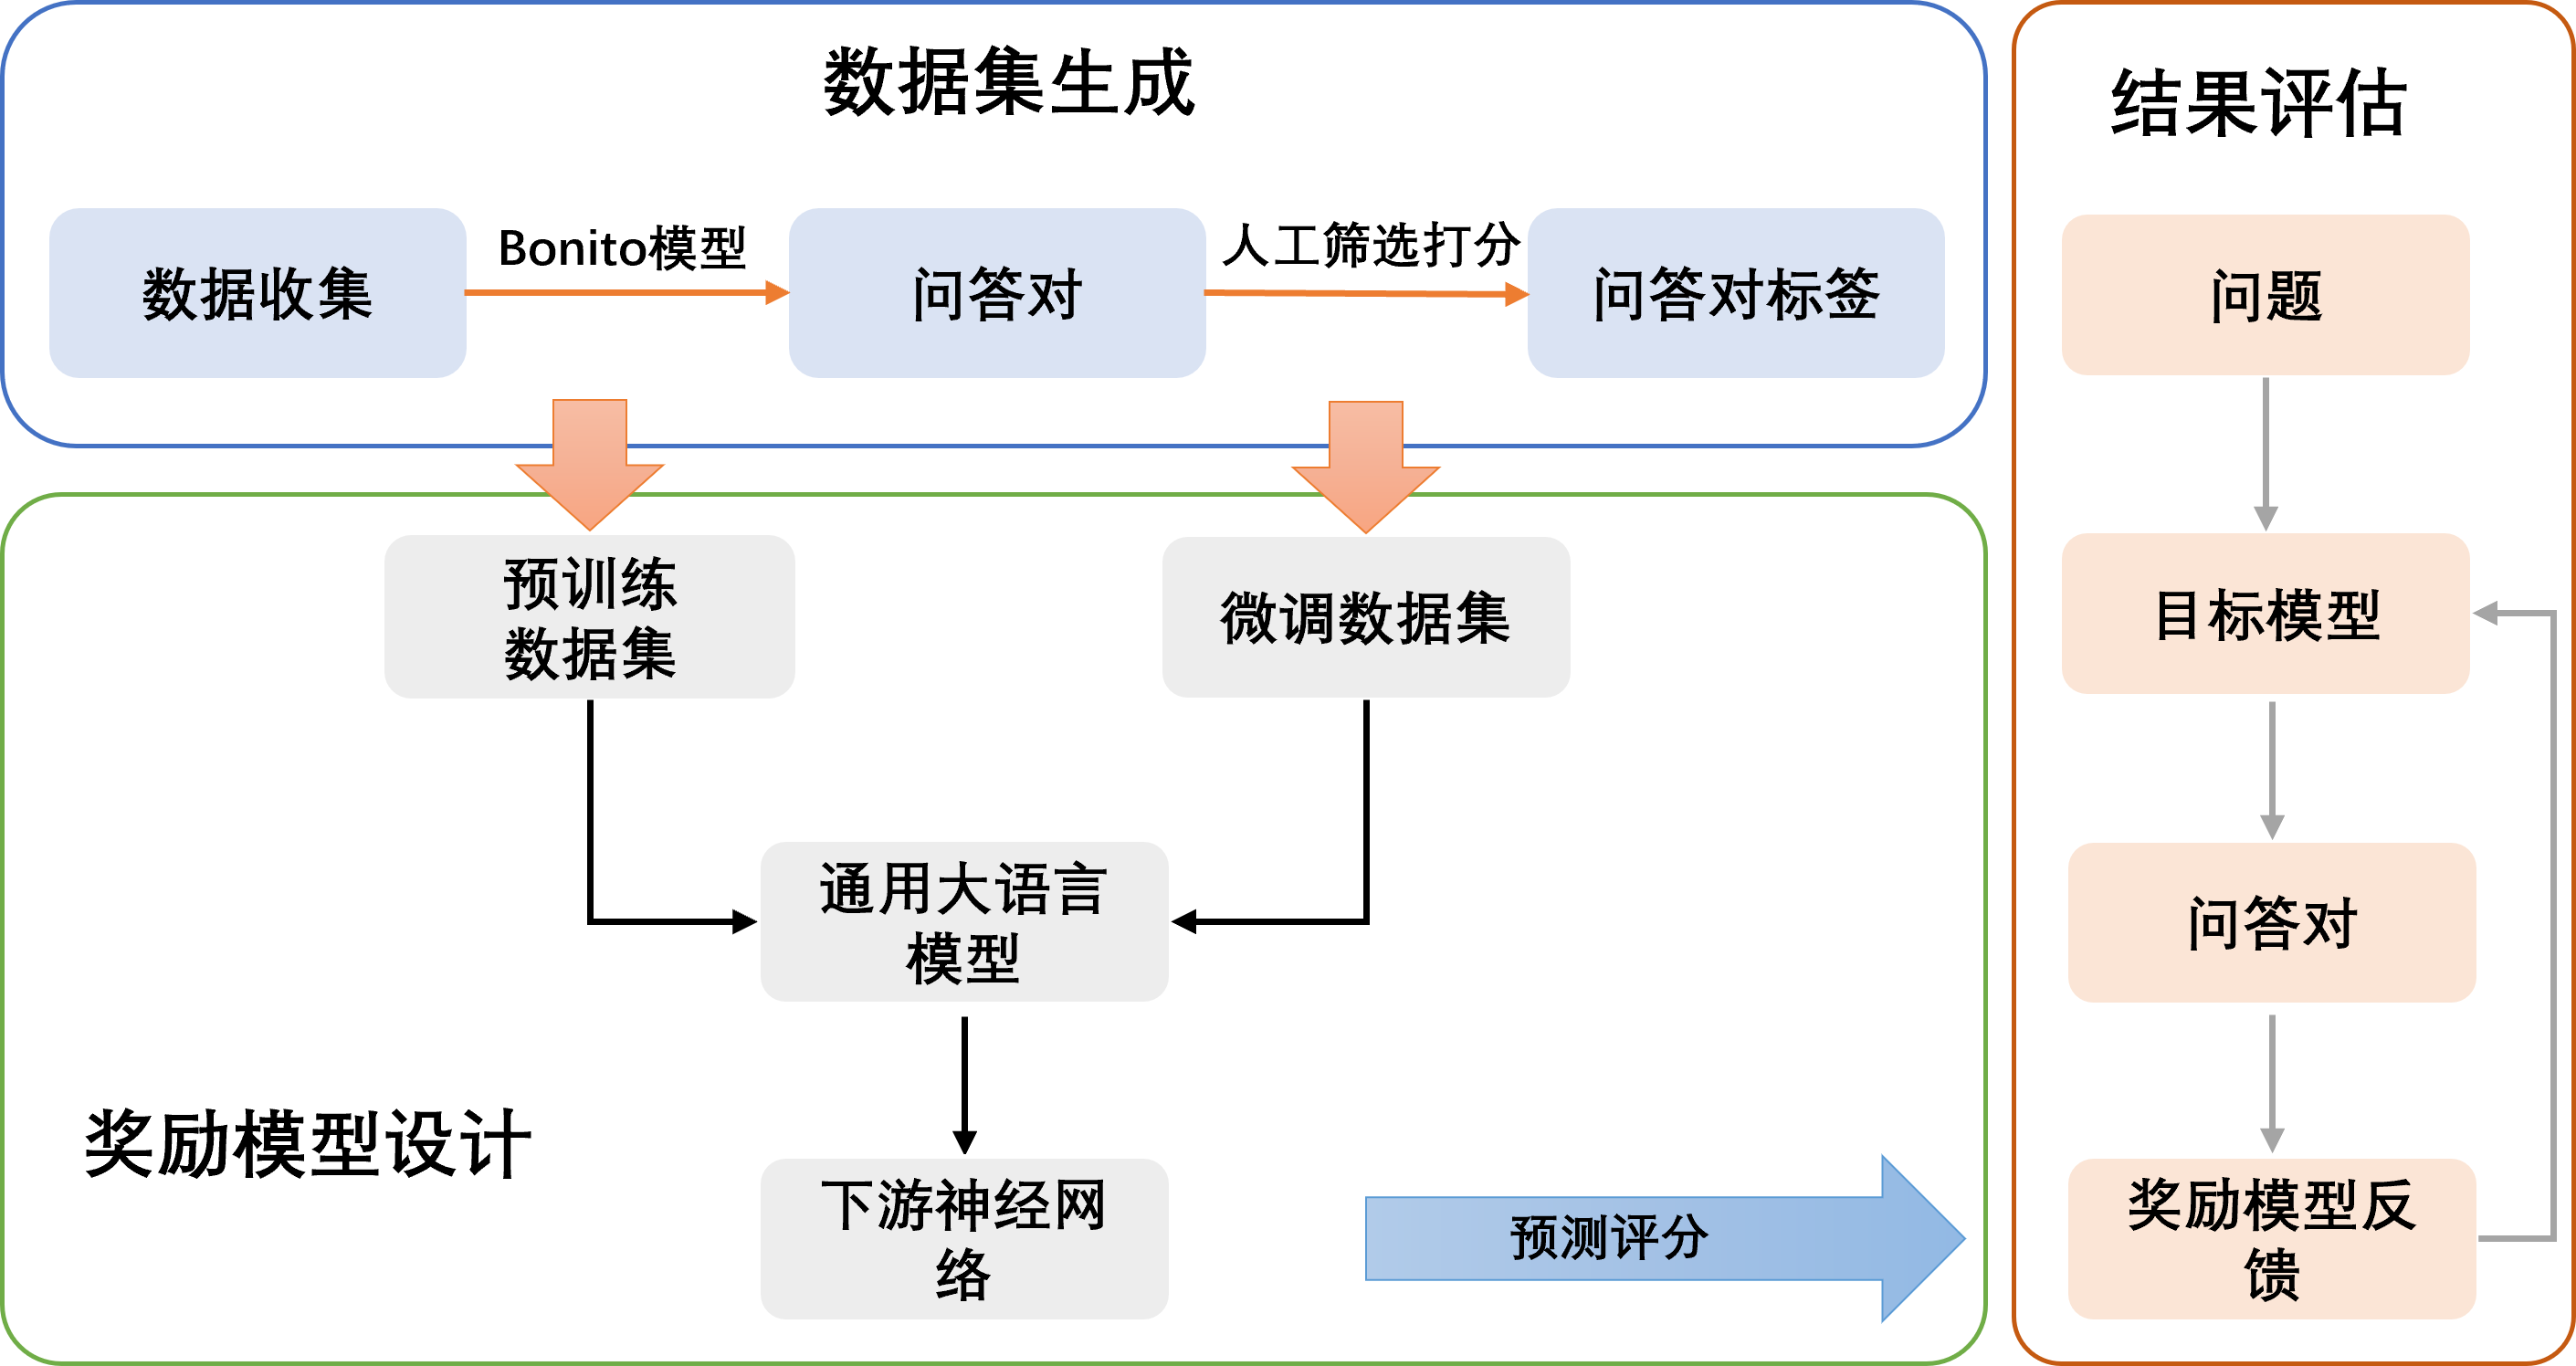
\includegraphics[width=0.9\textwidth]{./img/liucheng.png}
    \caption{研究方案}\label{fig:研究方案}
\end{figure}
\subsection{数据收集}
\begin{itemize}
    \item[1.] 网安文本:通过安全公司、研究机构和开源社区的恶意代码分析报告。以及其他平台AlienVault OTX、ThreatCrowd、Malware Information Sharing Platform (MISP)等。从公开的研究报告、白皮书、博客文章等获取情报数据。
    \item[2.] 网络爬虫:编写python脚本获取VirusTotal、MalwareBazaar、VirusShare、KDD Cup 99、NSL-KDD、CIC-IDS2017等数据集。
\end{itemize}
\subsection{Bonito模型}
由于问题是是-否类型,所以使用基于二分类的生成Bonito模型来生成一个问答对数据集,模型会将网络安全文本与问题类型标签作为输入,调整输出为问答对格式。
\subsection{指令微调}
将生成的问答对经过人工筛选和打分,即对于每一个样本,人为对Bonito模型生成的问答对添加评分标签。这些比较结果(即评分标签)同时会被用作训练数据,让奖励模型学习预测我们对模型的判断的偏好。而且与微调相比,指令微调需要的数据更少,适应速度更快\cite{pmlr-v202-longpre23a},指令直接解释需要改进的地方,如果需求发生变化,指令可以迭代,能够通过对话式指导。


\subsection{奖励模型}
由于FT只是将预训练模型中的知识给引导出来的一种手段,而在SFT数据有限的情况下,我们对模型的引导能力就是有限的。这将导致预训练模型中原先错误或有害的知识没能在SFT数据中被纠正,从而出现有害性或幻觉\cite{Ye2023CognitiveMA}的问题,从而在RLHF的过程中使用奖励模型。在进行RLHF时,需要奖励模型来评估语言大模型(actor model)回答的是好是坏,这个奖励模型通常比被评估的语言模型小一些(由于模型太大不够稳定,损失值很难收敛且小模型成本较低,因此,RM模型采用参数量较小的模型)。奖励模型的输入是prompt+answer的形式,让模型学会对prompt+answer进行打分。

\section{研究方案}
研究的具体流程共分成三个大部分:即指令集的构造、奖励模型的设计、对目标模型的调整。其中指令集的构造会通过任务指令+Bonito模型生成的问答对+参数高效微调等步骤完成,奖励模型的设计会通过奖励模型+人工反馈+参数高效微调等步骤完成,对目标模型的调整会通过奖励模型+强化学习与下游神经网络的结合等步骤完成。

\subsection{Bonito模型}
由于我们要将问题类型标签与网络安全的数据收集部分(以下简称网安文本)一同送入Bonito模型的输入端,所以要对Bonito的模型架构稍作调整。
\begin{figure}[htbp]
    \centering
    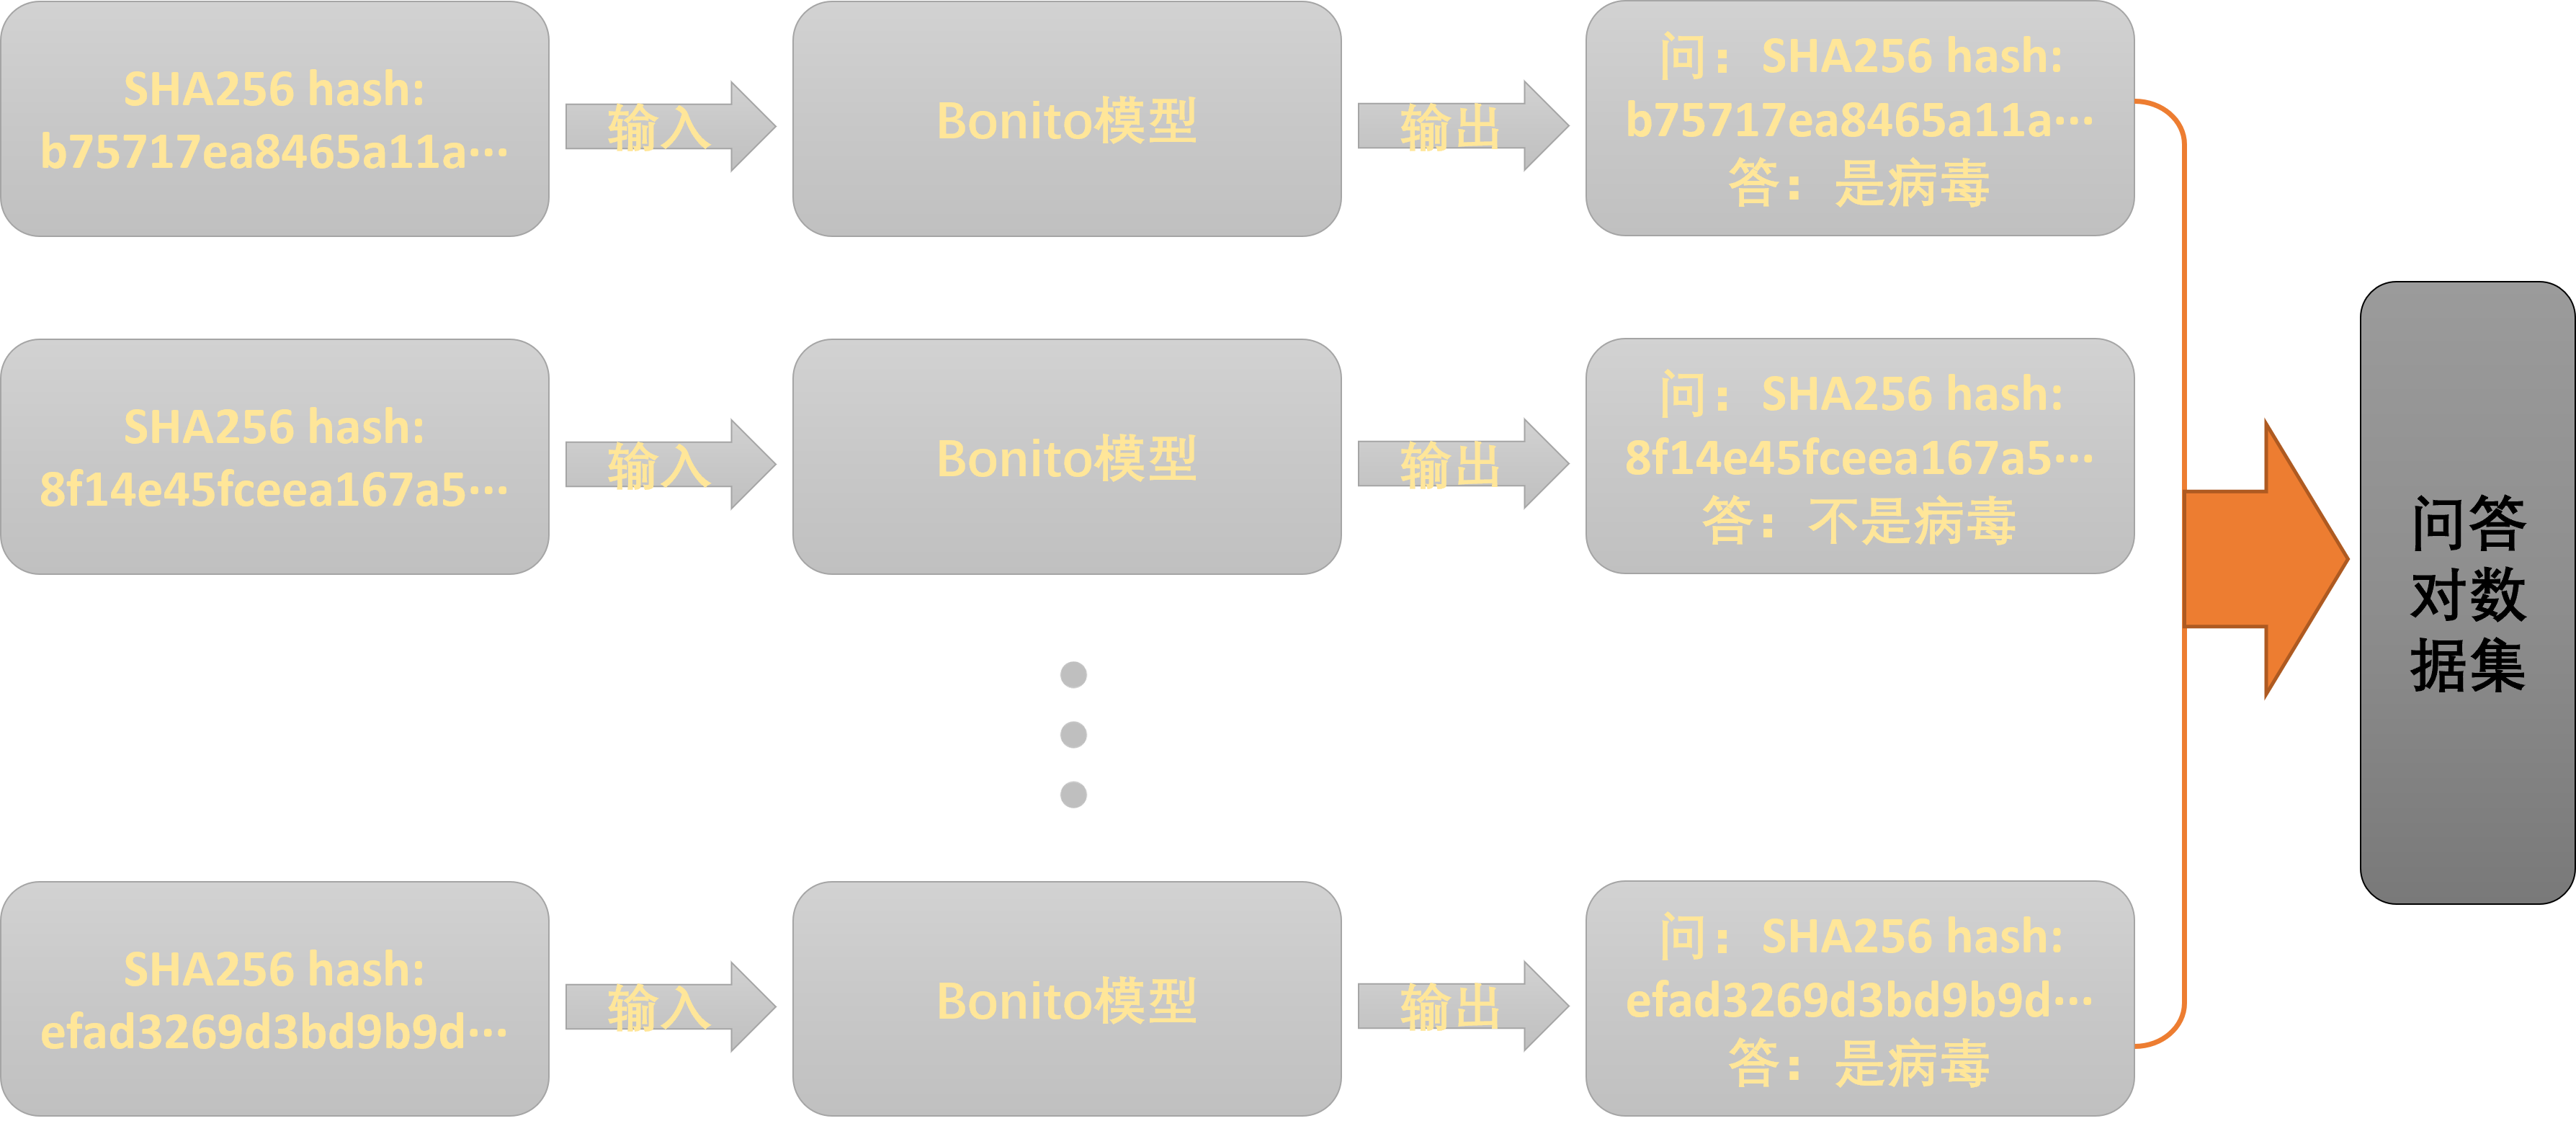
\includegraphics[width=0.8\textwidth]{./img/prompt.png}
    \caption{Bonito模型生成问答对流程}\label{fig:bonito}
\end{figure}

\begin{itemize}
    \item[1.] 数据预处理(输入):
    由于Bonito通常处理数值序列,将网络安全文本和问题类型标签转化为Bonito模型可以接受的输入序列,即将文本转换为数值表示:
        \begin{itemize}
            \item 字符级别的编码(每个字符映射为数字)。
            \item 使用词嵌入或预训练的文本编码器(如 Word2Vec、BERT 的嵌入)。
        \end{itemize}
        \item[2.]输出格式处理:输出也需要编码为Bonito可处理的问答对格式。
        \begin{figure}[htbp]
            \centering
            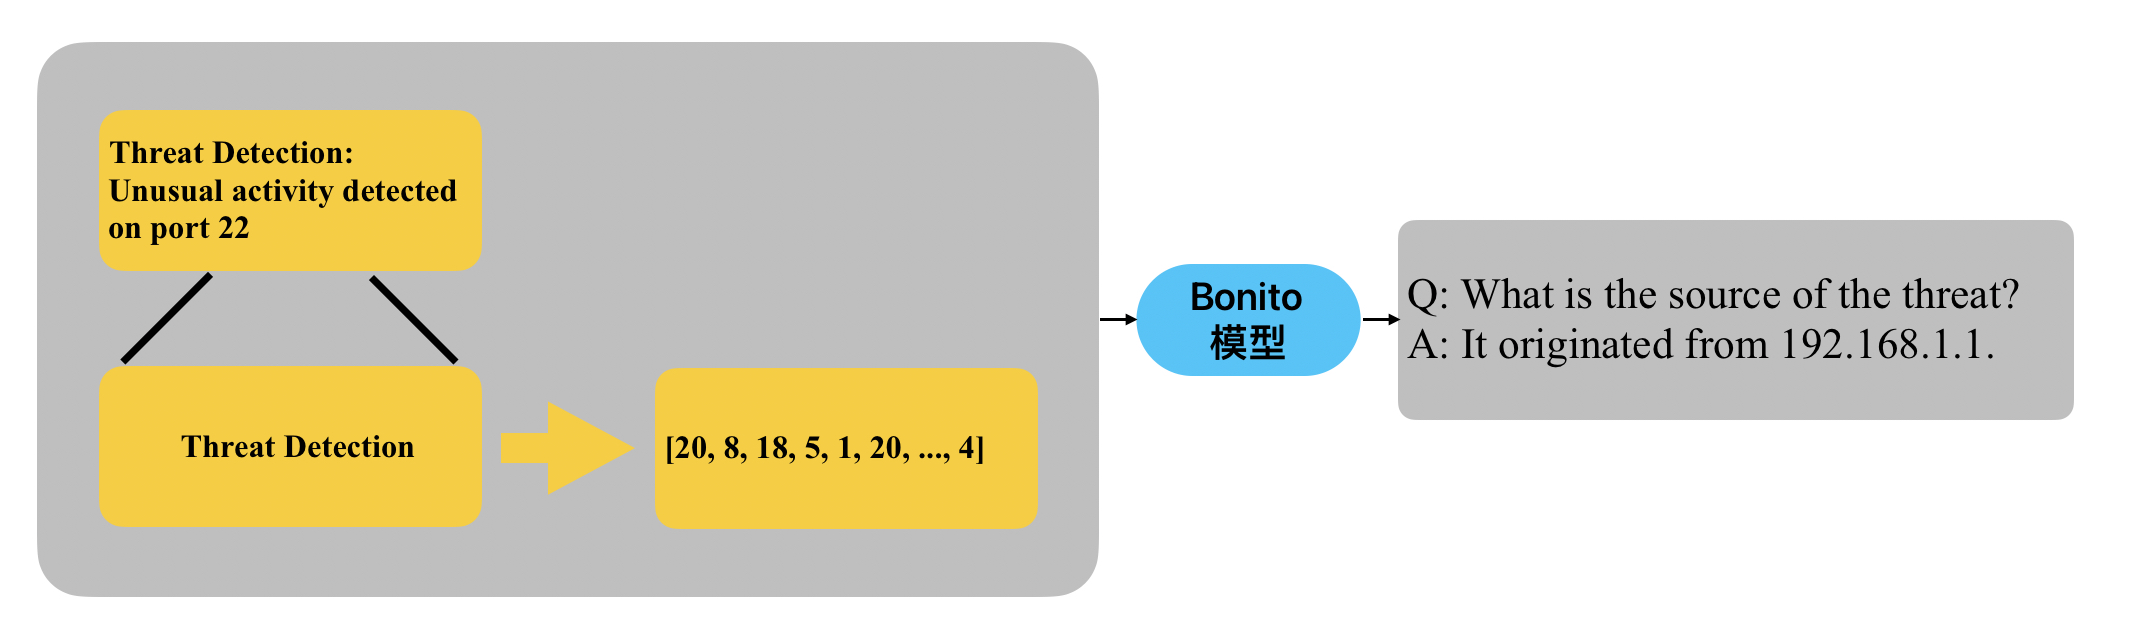
\includegraphics[width=0.8\textwidth]{./img/datadeal2.png}
            \caption{数据处理与问答对生成流程}\label{fig:bonito}
        \end{figure}
    利用Bonito模型从未标注的网络安全文本中生成合成任务数据集。可以通过创建条件任务生成模板(如“yes-no问题回答”),使模型从输入的文本中生成相应的任务指令和回答\cite{nayak-etal-2024-learning}​。
    \item[2.]修改Bonito模型:
    由于Bonito使用卷积神经网络和CTC解码器。为适配文本生成任务,需要以下调整:
    \begin{itemize}
        \item[1.]替换输出层:将输出层改为 Seq2Seq 生成任务中常用的Transformer解码器或LSTM解码器。通过通过自注意力机制能够更好地捕捉序列中的长距离依赖关系,这对于文本生成任务尤为重要,因为文本中往往存在跨越长距离的语义联系。
        \item[2.]增加注意力机制:Transformer解码器自带的注意力机制可以提升模型的生成能力,通过关注输入序列中与当前输出最相关的部分来生成更准确的文本。
        \item[3.]支持双通道输入:添加一个独立通道处理问题类型标签,并将问题类型标签嵌入与文本嵌入拼接做为输入。
    \end{itemize}
\end{itemize}
\subsection{指令微调奖励模型}
通过这些合成的问答对数据集与带评分标签的数据集,对预训练好的大规模语言模型进行有监督的微调,帮助LLM拥有更好的推理能力, 从而展现出泛化到未见过任务的卓越能力。也就是说,就算微调的指令中没有设计相关的任务,大模型在新任务上的表现也会优于微调之前\cite{nayak-etal-2024-learning}。
指令微调的目标是教模型根据网络安全文本和问题类型标签生成相关的问答对。指令集需要覆盖多种问题类型和场景,保证模型的泛化能力。
\begin{figure}[htbp]
    \centering
    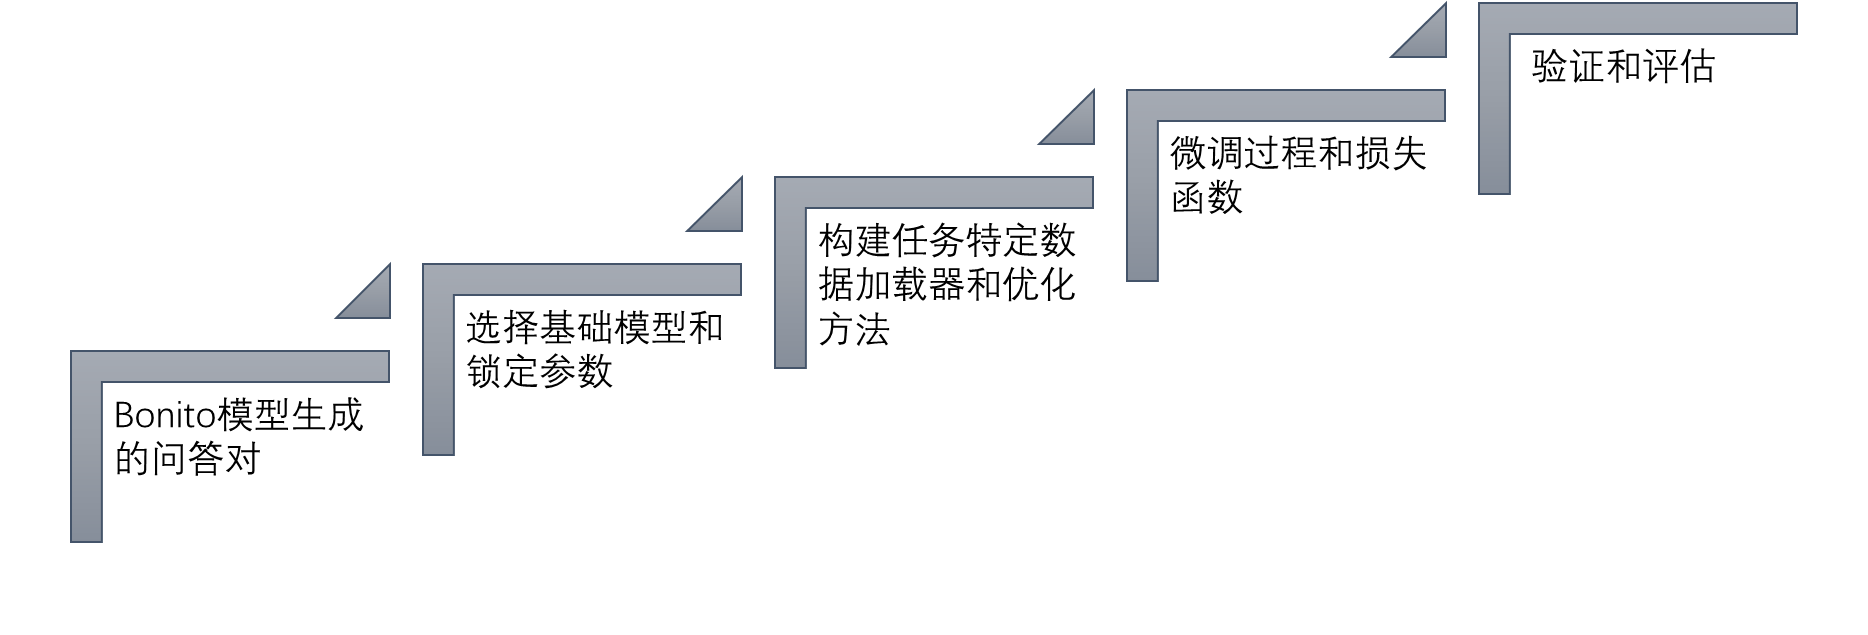
\includegraphics[width=0.8\textwidth]{./img/ft.png}
    \caption{指令微调过程}\label{fig:指令微调过程}
\end{figure}
\begin{itemize}
    \item [1.] 参数高效微调(Parameter-Efficient Fine-Tuning):由于LoRA\cite{2021LoRA}只对自注意力层的权重进行微调,而没有对线性层的权重进行微调,而奖励模型(RM模型)将SFT模型最后一层的softmax去掉,即最后一层不用softmax,改成一个线性层,所以LoRA并不适用于该任务。但是譬如FLAN2022、T5等大模型通常已经经过大量预训练,因此在指令微调时,通常只需微调部分参数\cite{li2021prefix},以确保模型保留通用语言能力并提高特定任务表现。也可以使用适配器进行指令微调\cite{hu-etal-2023-llm},从而减少模型修改的复杂性和成本。
    \item [2.]构建任务特定数据加载器和优化方法:使用 PyTorch 或 Hugging Face Transformers,可以将是否式问答对任务的数据转换为适合通用大语言模型的输入格式。在优化过程中,使用交叉熵损失函数来计算模型生成的答案和实际答案之间的差异。
          \begin{itemize}
              \item [i.]AdamW优化器\cite{hu-etal-2023-llm}:AdamW是适合微调大型语言模型的优化器,可以在训练中减少权重衰减(Weight Decay),有助于模型更好地泛化。
              \item [ii.]学习率调度:使用学习率调度器,如线性下降调度器(Linear Decay Scheduler),在训练过程中动态调整学习率,从而避免在微调时出现过度更新。
          \end{itemize}
    \item [3.]微调过程和损失函数设计:在微调过程中,输入模型的每一条数据应包括指令、上下文、问题和答案。微调使用损失函数计算生成的答案与真实答案的差距,并进行反向传播和参数更新。根据任务的流程,可以初步设计一个多层次的损失函数,例如:
          \begin{itemize}
              \item 正确性损失(Correctness Loss):衡量模型预测的评价与真实标注的正确性是否一致。
                    \begin{equation}
                        \mathcal{L}_{\text{correctness}} = -\sum_{i} y_{\text{true}, i} \log(y_{\text{pred}, i})
                    \end{equation}
                    其中 \( i \) 表示正确性评分的不同类别。
              \item 准确性损失(Accuracy Loss):使用均方误差(Mean Squared Error, MSE)来衡量模型预测的评分与真实标签评分之间的距离。准确性损失可以帮助模型更精确地对回答质量进行评分。
                    \begin{equation}
                        \mathcal{L}_{\text{accuracy}} = \frac{1}{N} \sum_{i=1}^{N} (y_{\text{true, accuracy}, i} - y_{\text{pred, accuracy}, i})^2
                    \end{equation}
                    其中 \( y_{\text{true, accuracy}, i} \) 表示回答的真实准确性评分,\( y_{\text{pred, accuracy}, i} \) 表示模型预测的准确性评分,\( N \) 为样本数量。
              \item 一致性损失:衡量模型对回答风格或格式的一致性评分与真实标注的匹配程度。
                    如果有关于回答一致性的评分(例如格式和风格是否符合预期),可以将其作为一个二分类任务来处理,使用二元交叉熵损失。
                    \begin{equation}
                        \mathcal{L}_{\text{consistency}} = - \left( y_{\text{true}} \log(y_{\text{pred}}) + (1 - y_{\text{true}}) \log(1 - y_{\text{pred}}) \right)
                    \end{equation}
                    其中 \( y_{\text{true}} \) 表示真实的一致性标签,\( y_{\text{pred}} \) 表示模型预测的一致性评分。
          \end{itemize}
          最终损失函数:
          \begin{equation}
              \mathcal{L} = \alpha \cdot \mathcal{L}_{\text{correctness}} + \beta \cdot \mathcal{L}_{\text{accuracy}} + \gamma \cdot \mathcal{L}_{\text{consistency}}
          \end{equation}
          \(\alpha\)、\(\beta\)、\(\gamma\)可以根据任务的具体需求进行调整。
\end{itemize}
\subsection{奖励模型的设计}
此处的通用大模型是用作奖励模型(Reward Model)来调整最终模型,大致的流程涉及上述的指令微调、奖励建模和强化学习(RLHF,Reinforcement Learning with Human Feedback)。奖励模型的反馈与下游神经网络相结合,通过强化学习的方法(如PPO\cite{Wang2024APT},Proximal Policy Optimization)来优化目标模型,以提升回答准确性。
\begin{figure}[htbp]
    \centering
    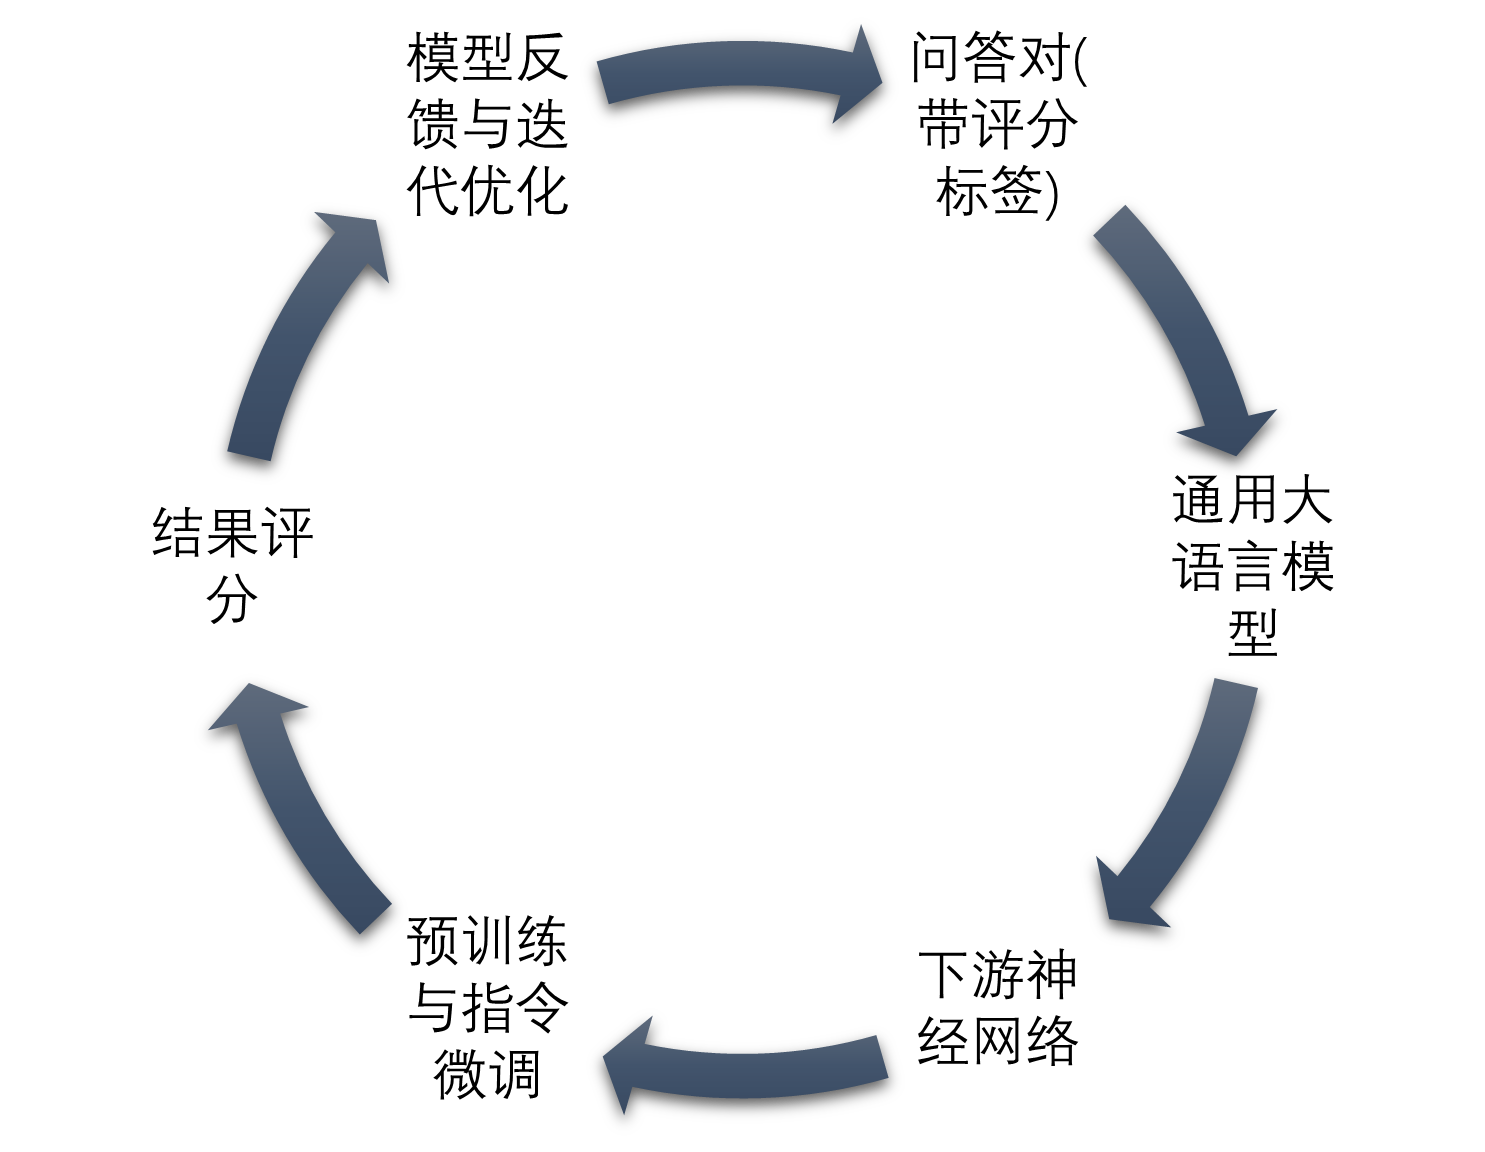
\includegraphics[width=0.45\textwidth]{./img/rm.png}
    \caption{奖励模型设计}\label{fig:奖励模型设计}
\end{figure}
\begin{itemize}
    \item[1.]奖励模型的输入设计\cite{pmlr-v202-longpre23a}:奖励模型的输入有三个:指令集、网安文本、带有评分标签的问答对,指令即为任务目标,为了提高模型的泛化能力,指令集要尽可能的丰富,输入中每一个网安文本对应的带有评分标签的问答对都会做为训练集。其中的文本嵌入过程可以使用SentencePiece分词器实现由文本到单词到编码序列到嵌入向量的过程。
    \item[2.]奖励模型的输出设计:由于奖励模型的目的是对目标模型的调整,调整方式为接受目标模型的输出的问答对与网安文本,所以奖励模型的输出为对该网安文本提出的问题的回答带上一个评分标签。由于奖励模型的输出要交给下游神经网络继续任务,所以采用最终隐藏状态输出较为合理,其形式为:\[ \text{[batch\_size, sequence\_length,  hidden\_size]} \]
    其中$\text{batch\_size}$是批次大小,$\text{sequence\_length}$是状态序列长度,$\text{hidden\_size}$是维度。
    \item[3.] 下游神经网络的设计\cite{Chung2022ScalingIL}:
    \begin{itemize}
        \item[1.]池化层设计:下游神经网络通过接受奖励模型的最终隐藏状态输出后要将其池化处理将序列数据转为定长做为全连接层的输入。池化层可选择平均池化捕捉序列中的全局信息。
        \[P_{\text{avg}}(i, j) = \frac{1}{K \times K} \sum_{m=0}^{K-1} \sum_{n=0}^{K-1} P_{\text{input}}(i + m, j + n)\]
        \item[2.]全连接层设计:通过多个线性层,将输出层的输出更改为一个做为评分的标量。
    \end{itemize}
\end{itemize}
\subsection{结果评估与闭环反馈}
奖励模型的设计通过反复的生成和反馈,逐步提升了目标模型的性能\cite{pmlr-v202-longpre23a}。在结果评估阶段,目标模型会利用奖励模型和人工标注的数据进行测试,以确保其能够有效处理各种类型的问题。通过奖励模型的持续反馈和人类评分之间的对比,进一步调整模型的生成逻辑与评估标准,形成一个完善的反馈回路闭环。
\begin{figure}[htbp]
    \centering
    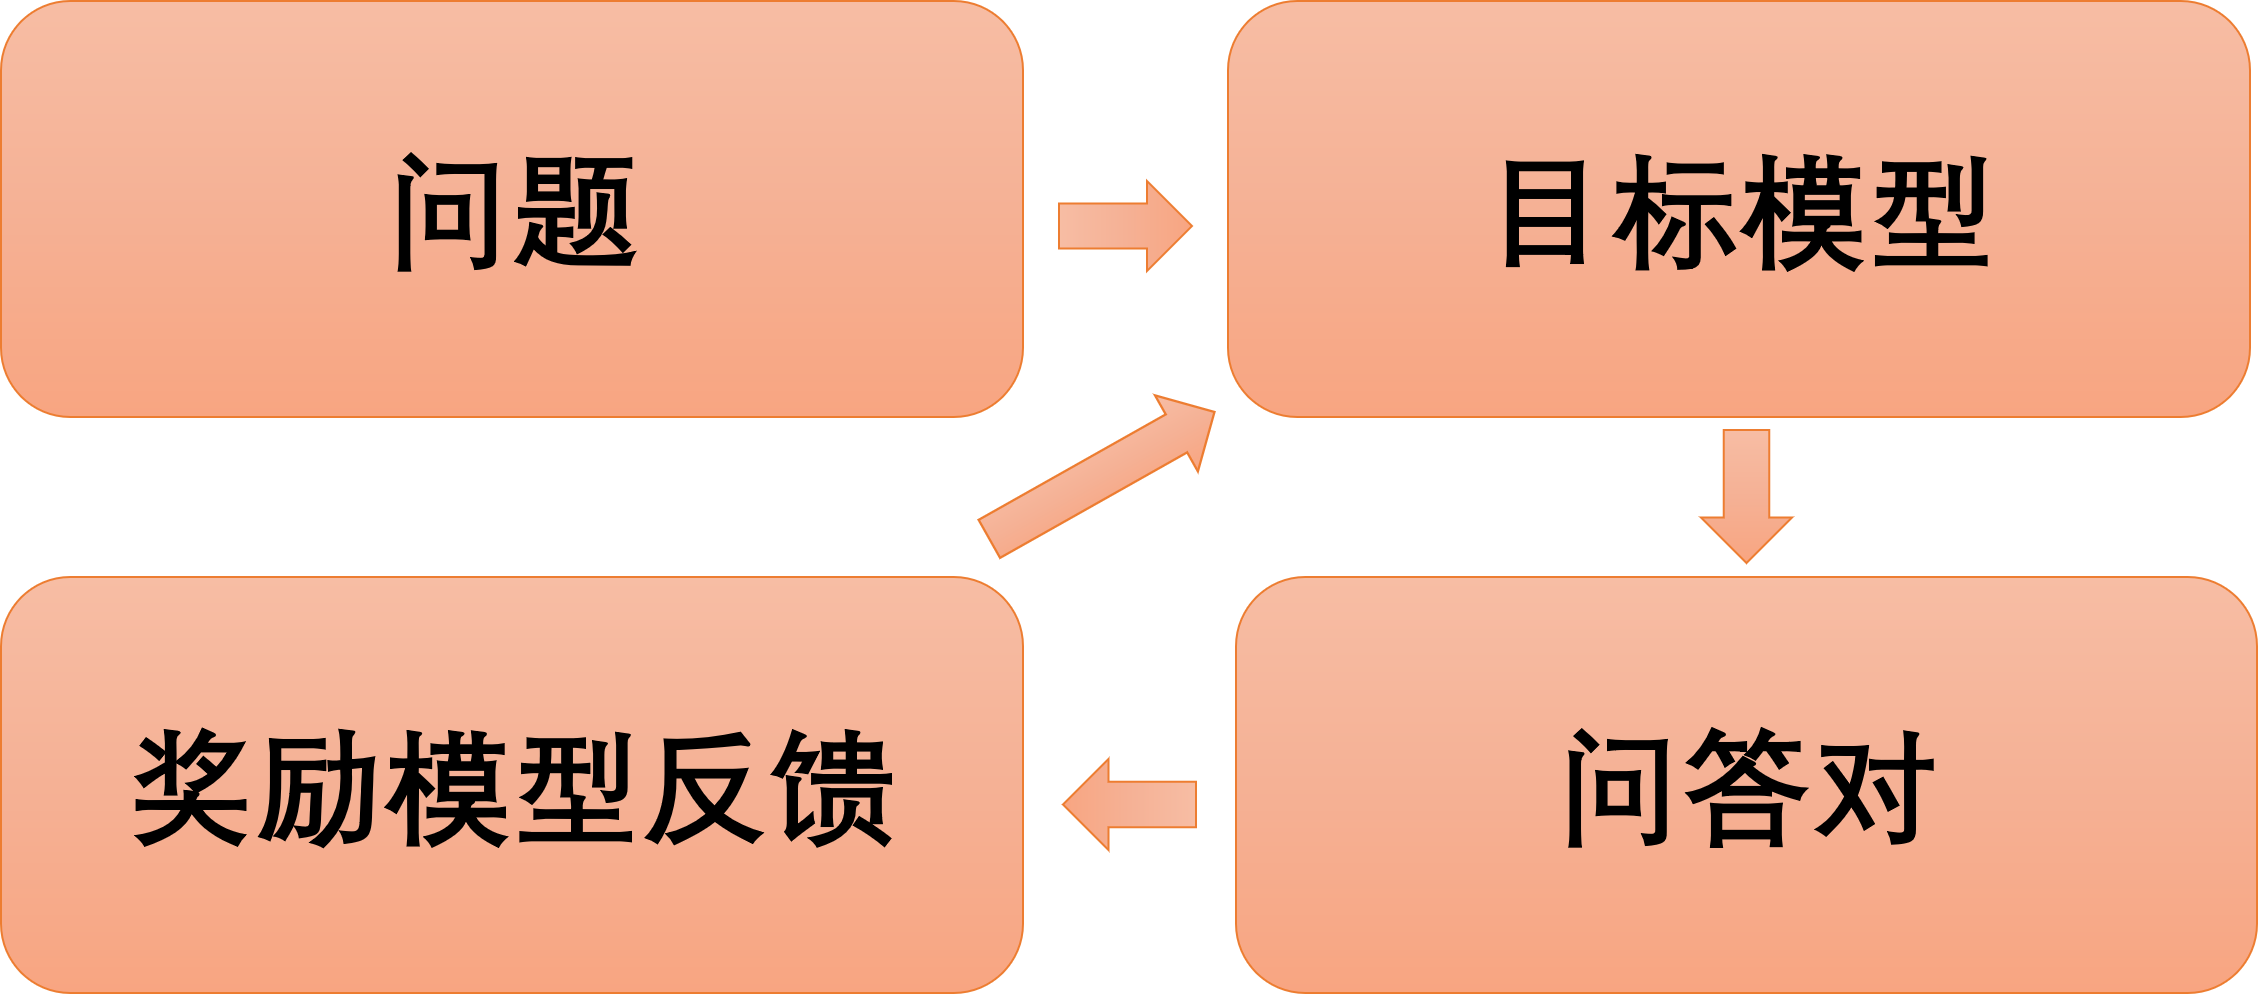
\includegraphics[width=0.35\textwidth]{./img/pre.png}
    \caption{奖励模型与目标模型的反馈循环}\label{fig:feedback_loop}
\end{figure}

\section{进度安排,预期达到的目标}
整个项目的进度安排与预期目标如下:
\begin{table}[htbp]
    \bicaption[table1]{}{项目任务时间表}{Table$\!$}{Timeline of project tasks}
    \vspace{0.5em}\centering\wuhao
    \begin{tabular}{ccccc}
        \toprule
        任务          & 时间              & 预期目标        \\
        \midrule
        爬虫开发与文本收集   & 24年11月-24年12月中旬 & 编写基本的爬虫代码   \\
        数据的预处理      & 24年11月-24年12月中旬 & 完成数据清洗和预处理  \\
        Bonito模型的设计 & 25年1月-25年2月中旬   & 完成初步问答对生成。  \\
        奖励模型设计与实现   & 25年3月-25年4月     & 对通用大模型指令微调  \\
        结果评估与反馈改进   & 25年4月-25年4月中旬   & 根据反馈对目标模型调整 \\
        \bottomrule
    \end{tabular}
\end{table}

\section{课题已具备和所需的条件、经费}
\begin{itemize}
    \item[1.] \textbf{已具备的条件:}
        \begin{itemize}
            \item \textbf{数据收集与预处理能力}:我在暑假期间完成了基本的网络爬虫工具以爬取一定数量的病毒样本,并继续对数据进行了清洗与预处理。
            \item \textbf{模型开发环境}:目前已经搭建个人模型开发环境:PyTorch深度学习框架。
        \end{itemize}
    \item[2.]\textbf{所需的条件:}
         \textbf{更多高质量的数据集}:为了提升问答对的质量,我需要收集和标注更多网络安全病毒样本的高质量数据集,尤其是最新的威胁情报、恶意代码分析报告等。
    \item[3.]\textbf{课题经费}:该课题预计没有经费支出。
\end{itemize}

\section{研究过程中可能遇到的困难和问题,解决的措施}
\subsection{Bonito模型数据不平衡}
网络安全数据可能存在类别不平衡,即正常样本和恶意样本的数量差异很大,这可能导致模型偏向于预测多数类。

解决方法:
\begin{itemize}
    \item[1.] SMOTE\cite{10.5555/1622407.1622416}
        (合成少数类过采样技术):可以通过SMOTE方法对少数类进行过采样。SMOTE通过在少数类样本之间生成新的合成样本,而不是简单地重复现有样本,避免了过拟合问题。例如,选择少数类样本的最近邻\cite{2005Borderline},然后在样本之间随机生成新的数据点,这样可以扩大少数类数据的表示范围,从而更好地平衡数据集。由于SMOTE对所有少数类样本平等对待,可能会在某些区域生成过多的合成样本,这增加了过拟合的风险。
    \item[2.] 数据清洗与采样:可以使用欠采样方法\cite{Krawczyk2016LearningFI},从多数类中随机删除部分样本,或者结合过采样与欠采样的方法,通过清洗掉噪声样本和难以区分的边界样本来平衡数据集。例如,边界样本可以通过最近邻算法来识别,这样有助于去除对模型性能有负面影响的样本​。
\end{itemize}

\subsection{模型过拟合问题}
网络安全数据可能包含大量噪声和冗余信息,这可能导致模型过拟合训练数据。并且模型可能在训练集上表现良好,但在未见过的数据上表现不佳。

解决方法:
\begin{itemize}
    \item[1.] 正则化:在模型训练过程中,可以通过添加正则化项(如L1或L2正则化)来防止过拟合。正则化项会惩罚模型参数的大小,从而限制模型的复杂度\cite{10533733}。例如,在神经网络中,可以通过在损失函数中添加L2正则化\cite{10.1145/2347736.2347755}项来防止过拟合。\item[2.]加入Dropout层\cite{Cai2019EffectiveAE}。Dropout通过随机去除部分神经元来减少模型的复杂性,从而降低过拟合的风险。L2正则化通过在损失函数中添加参数权重的平方惩罚项,限制权重的过大值,这有助于提高模型的泛化能力。
        \begin{figure}[htbp]
            \centering
            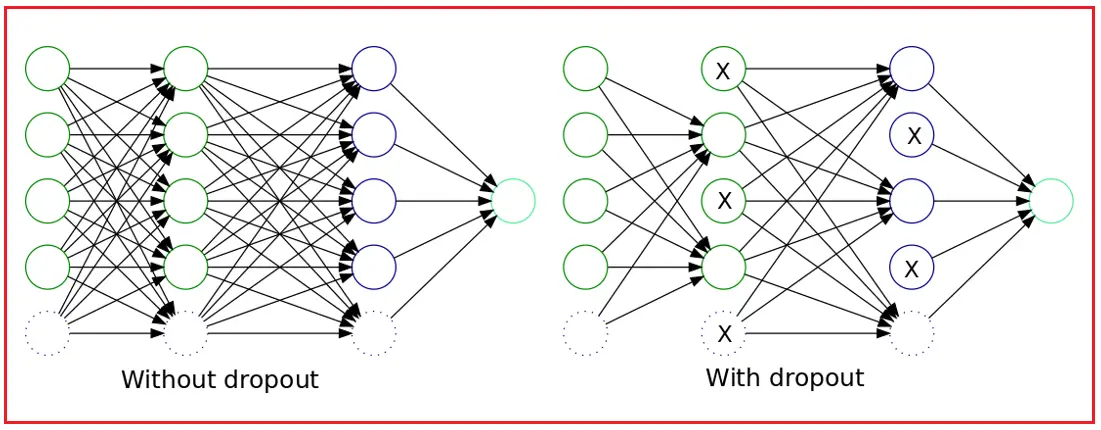
\includegraphics[width=.9\textwidth]{./img/dropout.png}
            \caption{应用Dropout后的神经网络}\label{img2}
        \end{figure}
    \item[3.] 交叉验证:利用交叉验证来评估模型的泛化误差。例如,使用k折交叉验证\cite{10533733}来评估模型在不同数据划分上的表现,以检测过拟合现象。这种方法有助于确保模型不会仅仅学习训练数据,而且加强对未见数据的泛化能力​。
\end{itemize}

\section{主要参考文献}
\bibliographystyle{hithesis}
\bibliography{reference}

% Local Variables:
% TeX-master: "../mainart"
% TeX-engine: xetex
% End: